% ---
% titre: Calculs de priorités des opérations (séries A, B et C)
% theme: NO
% chapitre: Nombres naturels et décimaux
% sous_chapitre: Priorité des opérations
% niveau: [10e,11e]
% type: EX
% tags: [c-priorite-operations, f-individuel,f-maison,f-station,p-entrainement,p-remediation]
% difficulte: 3
% source: latex
% ---

\header{Additions et soustractions de nombres relatifs}

{\small
\bigskip
\def\arraystretch{1.7}
\begin{tabularx}{\linewidth}{*{4}{X}}
\textbf{A.} & \textbf{B.} & \textbf{C.} & \textbf{D.} \\
$(+8)+(-3)= \sol{\dotfill}{+5}$   & $(-5)+(+9)= \sol{\dotfill}{+4}$   & $(+10)+(-14)= \sol{\dotfill}{-4}$ & $(-3)-(+9)= \sol{\dotfill}{-12}$   \\
$(+6)-(+12)= \sol{\dotfill}{-6}$  & $(+14)+(-19)= \sol{\dotfill}{-5}$ & $(-10)+(-12)= \sol{\dotfill}{-22}$ & $(+8)-(-8)= \sol{\dotfill}{+16}$   \\
$(+4)+(+11)= \sol{\dotfill}{+15}$  & $(-17)-(-15)= \sol{\dotfill}{-2}$ & $(+9)+(-9)= \sol{\dotfill}{0}$   & $(+24)-(+14)= \sol{\dotfill}{+10}$ \\
$(-24)-(+12)= \sol{\dotfill}{-36}$ & $(+9)+(+13)= \sol{\dotfill}{+22}$  & $(-12)+(-8)= \sol{\dotfill}{-20}$  & $(-14)+(-7)= \sol{\dotfill}{-21}$  \\
$(+15)-(-7)= \sol{\dotfill}{+22}$  & $(+10)-(-9)= \sol{\dotfill}{+19}$  & $(+14)+(-5)= \sol{\dotfill}{-9}$  & $(-15)-(-17)= \sol{\dotfill}{+2}$ \\
$(+14)+(-8)= \sol{\dotfill}{+6}$  & $(+12)-(-1)= \sol{\dotfill}{+13}$  & $(-5)-(-14)= \sol{\dotfill}{+9}$  & $(+20)-(+18)= \sol{\dotfill}{+2}$ \\
\end{tabularx}
}

\header{Simplification d'écriture et somme algébrique}

{\bfseries\color{themeColor}Exercice 1.} \quad$(+7) + (−4)−(+5) + (−6) + (+8)−(−9) =$

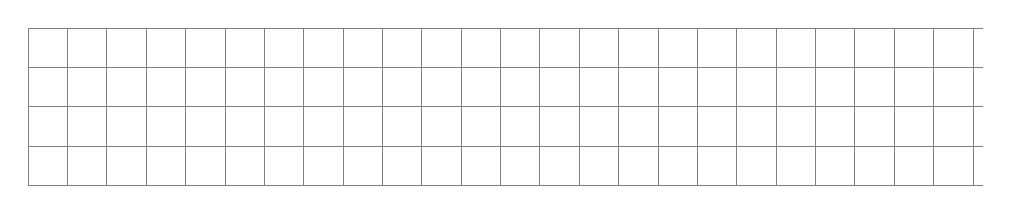
\begin{tikzpicture}\draw[step=0.5cm, gray, very thin] (0,0) grid (\textwidth,2);\end{tikzpicture}

{\bfseries\color{themeColor}Exercice 2.} \quad$(−12) + (+3)−(−5) + (+7)−(+9) + (−4) =$

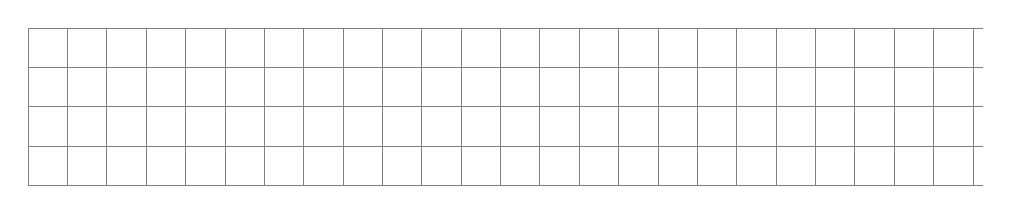
\begin{tikzpicture}\draw[step=0.5cm, gray, very thin] (0,0) grid (\textwidth,2);\end{tikzpicture}

{\bfseries\color{themeColor}Exercice 3.} \quad$(−35)−(+12) + (−23)−(−35) + (+40)$

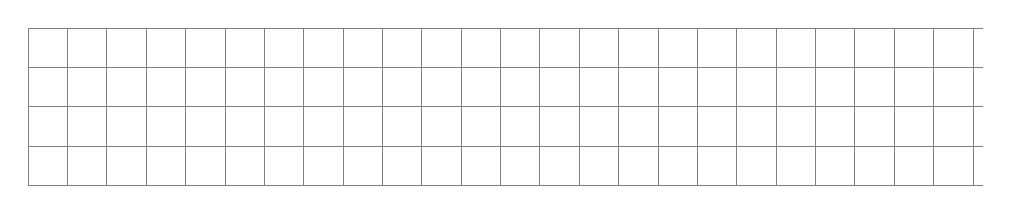
\begin{tikzpicture}\draw[step=0.5cm, gray, very thin] (0,0) grid (\textwidth,2);\end{tikzpicture}

{\bfseries\color{themeColor}Exercice 4.} \quad$(−20) + (−15)−(−10)−(−5) + (+12) + (+8) =$

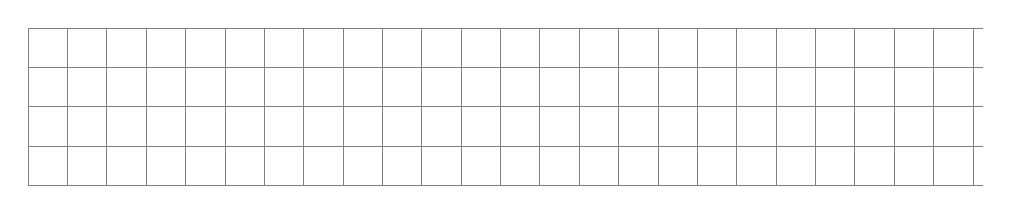
\begin{tikzpicture}\draw[step=0.5cm, gray, very thin] (0,0) grid (\textwidth,2);\end{tikzpicture}

{\bfseries\color{themeColor}Exercice 5.} \quad$(+16)−(−18) + (−22) + (−16) + (+14)−(−24) =$

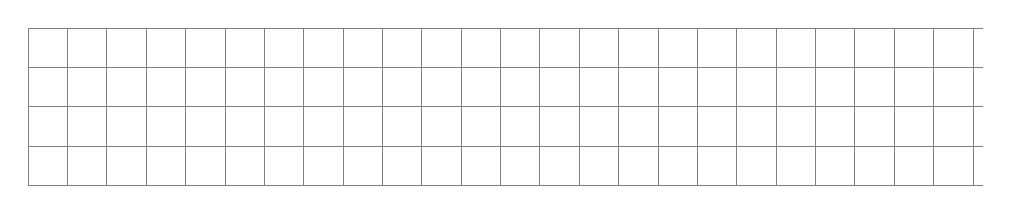
\begin{tikzpicture}\draw[step=0.5cm, gray, very thin] (0,0) grid (\textwidth,2);\end{tikzpicture}

{\bfseries\color{themeColor}Exercice 6.} \quad$(−8) + (+6)−(−7) + (+11)−(−2) =$

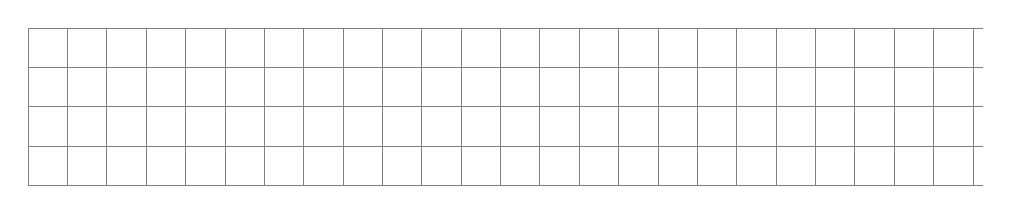
\begin{tikzpicture}\draw[step=0.5cm, gray, very thin] (0,0) grid (\textwidth,2);\end{tikzpicture}

{\bfseries\color{themeColor}Exercice 7.} \quad$(−13) + (+5)−(+7) + (−9)−(−11) + (+13) =$

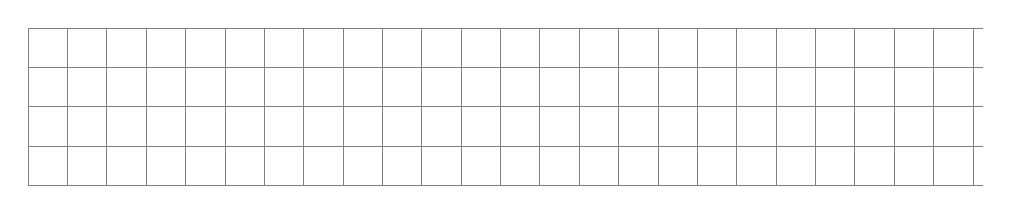
\begin{tikzpicture}\draw[step=0.5cm, gray, very thin] (0,0) grid (\textwidth,2);\end{tikzpicture}

{\bfseries\color{themeColor}Exercice 8.} \quad$(−6) + (−8)−(+4) + (+3)−(−2) + (+9) =$

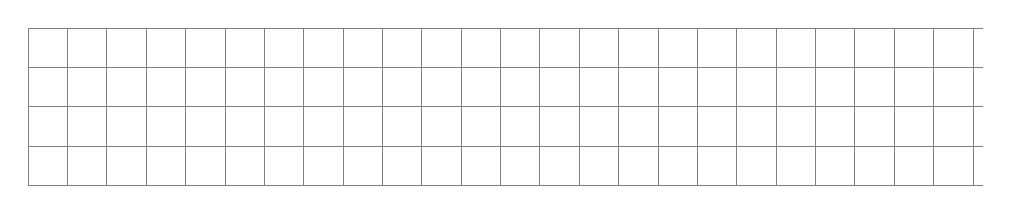
\begin{tikzpicture}\draw[step=0.5cm, gray, very thin] (0,0) grid (\textwidth,2);\end{tikzpicture}

{\bfseries\color{themeColor}Exercice 9.} \quad$(−24) + (−16)−(−8)−(+12) + (+32) =$

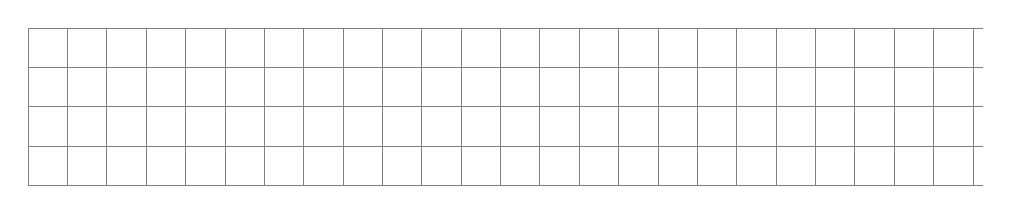
\begin{tikzpicture}\draw[step=0.5cm, gray, very thin] (0,0) grid (\textwidth,2);\end{tikzpicture}

{\bfseries\color{themeColor}Exercice 10.} \quad$(+10)−(+7)−(−9) + (−8) + (+6)−(−10) =$

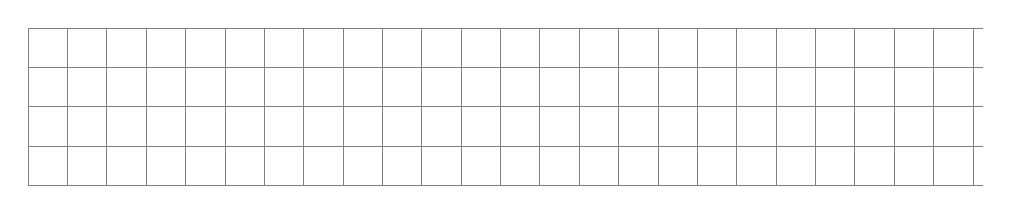
\begin{tikzpicture}\draw[step=0.5cm, gray, very thin] (0,0) grid (\textwidth,2);\end{tikzpicture}


\vfill
\header{Multiplications et divisions de nombres relatifs}

{\small
\bigskip
\def\arraystretch{1.7}
\begin{tabularx}{\linewidth}{*{4}{X}}
\textbf{A.} & \textbf{B.} & \textbf{C.} & \textbf{D.} \\
$(+5)\cdot(-3)= \dotfill$    & $(-45):(+5)= \dotfill$  & $(+56):(-7)= \dotfill$      & $(+27):(+9)= \dotfill$      \\
$(+6)\cdot(+12)= \dotfill$   & $(-14):(-7)= \dotfill$  & $(-10)\cdot(-11)= \dotfill$ & $(+4)\cdot(-8)= \dotfill$   \\
$(+8)\cdot(+11)= \dotfill$   & $(+90):(-10)= \dotfill$ & $(+9)\cdot(-9)= \dotfill$   & $(-63):(+7)= \dotfill$      \\
$(+42):(-7)= \dotfill$       & $(-72):(+12)= \dotfill$ & $(-12):(-4)= \dotfill$      & $(+11)\cdot(-11)= \dotfill$ \\
$(+96):(-12)= \dotfill$      & $(+6)\cdot(-4)= \dotfill$ & $(+25):(-5)= \dotfill$    & $(-49):(-7)= \dotfill$      \\
$(+48):(-8)= \dotfill$       & $(+28):(+7)= \dotfill$  & $(-5)\cdot(-6)= \dotfill$   & $(+10):(-10)= \dotfill$     \\
\end{tabularx}
}

\newpage
\header{C’est en forgeant que l’on devient forgeron !}

{\small
\bigskip
\def\arraystretch{1.2}
\begin{tabularx}{\linewidth}{*{4}{X}}
\textbf{A.} & \textbf{B.} & \textbf{C.} & \textbf{D.} \\
$(+14)-(-26)= \dotfill$ & $(-21)\cdot(+8)= \dotfill$ & $(-14)+(+12)= \dotfill$ & $(-7)+(+22)= \dotfill$ \\
$(+34)+(-48)= \dotfill$ & $(-25)\cdot(-5)= \dotfill$ & $(+150)+(-50)= \dotfill$ & $(+60)+(-25)= \dotfill$ \\
$(+21)\cdot(-9)= \dotfill$ & $(+180):(-6)= \dotfill$ & $(+200)-(-140)= \dotfill$ & $(+51)-(-75)= \dotfill$ \\
$(-145):(-5)= \dotfill$ & $(-36):(+9)= \dotfill$ & $(+36)+(-4)= \dotfill$ & $(-45)-(-35)= \dotfill$ \\
$(+38)+(-57)= \dotfill$ & $(+76)+(-41)= \dotfill$ & $(-20)\cdot(+55)= \dotfill$ & $(-8)\cdot(+7)= \dotfill$ \\
$(+24)\cdot(-4)= \dotfill$ & $(-47)+(+74)= \dotfill$ & $(+480)+(-12)= \dotfill$ & $(-13)\cdot(-7)= \dotfill$ \\
$(+55)-(+27)= \dotfill$ & $(-33)-(+65)= \dotfill$ & $(+180)+(-120)= \dotfill$ & $(-132):(-11)= \dotfill$ \\
$(-80):(+5)= \dotfill$ & $(+37)-(+22)= \dotfill$ & $(-38):(-19)= \dotfill$ & $(+72):(-9)= \dotfill$ \\
\end{tabularx}

\bigskip
\begin{tabularx}{\linewidth}{*{4}{X}}
\textbf{E.} & \textbf{F.} & \textbf{G.} & \textbf{H.} \\
$(+74)-(-16)= \dotfill$ & $(-22)\cdot(+7)= \dotfill$ & $(-18)+(+12)= \dotfill$ & $(-27)+(-22)= \dotfill$ \\
$(+24)+(-28)= \dotfill$ & $(-15)\cdot(-8)= \dotfill$ & $(-18)+(+32)= \dotfill$ & $(-15)+(+25)= \dotfill$ \\
$(-15)\cdot(+8)= \dotfill$ & $(+130):(-5)= \dotfill$ & $(+28)+(+42)= \dotfill$ & $(-150)+(+125)= \dotfill$ \\
$(-40):(-20)= \dotfill$ & $(-56):(+8)= \dotfill$ & $(-36)+(-12)= \dotfill$ & $(-45)+(-25)= \dotfill$ \\
$(+28)+(-46)= \dotfill$ & $(+26)+(-21)= \dotfill$ & $(+38)+(+36)= \dotfill$ & $(+58)+(+65)= \dotfill$ \\
$(+14)\cdot(-7)= \dotfill$ & $(-37)+(+64)= \dotfill$ & $(-48)+(-52)= \dotfill$ & $(-66)+(+120)= \dotfill$ \\
$(+35)-(+17)= \dotfill$ & $(-43)-(-72)= \dotfill$ & $(+180)+(-120)= \dotfill$ & $(-170)+(+75)= \dotfill$ \\
$(+70):(-2)= \dotfill$ & $(+45)-(+29)= \dotfill$ & $(-180):(+12)= \dotfill$ & $(+67)+(+52)= \dotfill$ \\
\end{tabularx}

\bigskip
\begin{tabularx}{\linewidth}{*{4}{X}}
\textbf{I.} & \textbf{J.} & \textbf{K.} & \textbf{L.} \\
$(+13)-(-16)= \dotfill$ & $(-12)\cdot(-11)= \dotfill$ & $(-18)+(-12)= \dotfill$ & $(-72)+(-42)= \dotfill$ \\
$(+23)-(-86)= \dotfill$ & $(-20)\cdot(-4)= \dotfill$ & $(+28)+(-42)= \dotfill$ & $(-25)+(+85)= \dotfill$ \\
$(-13)-(-26)= \dotfill$ & $(-13)\cdot(-13)= \dotfill$ & $(-48)+(+17)= \dotfill$ & $(-160)+(+145)= \dotfill$ \\
$(+40)-(+20)= \dotfill$ & $(-8)\cdot(+12)= \dotfill$ & $(+82)+(+54)= \dotfill$ & $(-145)+(+36)= \dotfill$ \\
$(+43)-(-16)= \dotfill$ & $(+140)\cdot(-6)= \dotfill$ & $(-63)+(-31)= \dotfill$ & $(+98)+(+25)= \dotfill$ \\
$(+30)-(+21)= \dotfill$ & $(-13)\cdot(-8)= \dotfill$ & $(+68)+(+36)= \dotfill$ & $(-86)+(+167)= \dotfill$ \\
$(-63)-(-12)= \dotfill$ & $(+15)\cdot(-4)= \dotfill$ & $(-58)+(+67)= \dotfill$ & $(-185)+(+73)= \dotfill$ \\
$(-53)-(-36)= \dotfill$ & $(-16)\cdot(-6)= \dotfill$ & $(+190)+(-130)= \dotfill$ & $(+97)+(+38)= \dotfill$ \\
\end{tabularx}

\bigskip
\begin{tabularx}{\linewidth}{*{4}{X}}
\textbf{M.} & \textbf{N.} & \textbf{O.} & \textbf{P.} \\
$(-23)+(-61)= \dotfill$ & $(-29)+(+67)= \dotfill$ & $(-17)-(+18)= \dotfill$ & $(+58)-(-49)= \dotfill$ \\
$(+130)\cdot(-4)= \dotfill$ & $(+43)+(+87)= \dotfill$ & $(-1)\cdot(+120)= \dotfill$ & $(-69)+(+35)= \dotfill$ \\
$(+3)\cdot(-69)= \dotfill$ & $(-84)-(-91)= \dotfill$ & $(+12)+(-87)= \dotfill$ & $(-55):(-5)= \dotfill$ \\
$(-73):(+10)= \dotfill$ & $(-66)-(-28)= \dotfill$ & $(-108):(-9)= \dotfill$ & $(-169)+(-7)= \dotfill$ \\
$(+19):(-0{,}5)= \dotfill$ & $(+13)\cdot(+6)= \dotfill$ & $(-27)-(+27)= \dotfill$ & $(-72)\cdot(-20)= \dotfill$ \\
$(-81)+(+48)= \dotfill$ & $(-97)\cdot(+30)= \dotfill$ & $(-96):(+4)= \dotfill$ & $(+12)\cdot(+60)= \dotfill$ \\
$(-31)-(+65)= \dotfill$ & $(-57):(-2)= \dotfill$ & $(+124)+(-135)= \dotfill$ & $(+92)-(-8)= \dotfill$ \\
$(-13)-(-86)= \dotfill$ & $(+232):(-116)= \dotfill$ & $(-18)\cdot(-6)= \dotfill$ & $(-169)+(-13)= \dotfill$ \\
\end{tabularx}}